\documentclass[border=3mm]{standalone}

\usepackage{tikz}
\usetikzlibrary{arrows,shapes.gates.logic.US,shapes.gates.logic.IEC,calc}
\begin{document}
\thispagestyle{empty}
\tikzstyle{branch}=[fill,shape=circle,minimum size=15pt,inner sep=0pt]
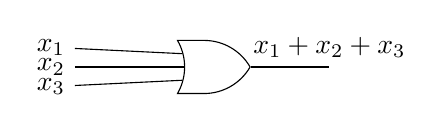
\begin{tikzpicture}[label distance=2mm]

    \node (x1) at (0,-0.25) {$x_1$};
    \node (x2) at (0,-.5) {$x_2$};
    \node (x3) at (0,-0.75) {$x_3$};

    \node[or gate US, draw, logic gate inputs=nnn] at (2,-0.5) (Or1) {};

    \draw (x1) -- (Or1.input 1);
    \draw (x2) -- (Or1.input 2);
    \draw (x3) -- (Or1.input 3);
    \draw (Or1.output) -- ([xshift=1.0cm]Or1.output) node[above] {$x_1 + x_2 +x_3$};
\end{tikzpicture}
\end{document} 
